\chapter{Troubleshooting}\label{cha:troubleshooting}

This section describes some problems that could be met with the user interface or some error messages displayed by QDOAS.  Most of error messages come from a wrong configuration (calibration or analysis settings).   If you can not solve a problem or if you have detected a bug, it's important to contact authors.  The log file produced by QDOAS in the application directory is an important source of information for us.  A small application with a detailed description of the trouble and the sequence of manipulations leading to it can help us to solve the problem quickly.

\section{Known user interface problems}

\subsection{Refreshing Problem In The Projects Properties}\hfill
\begin{figure}[!h]
\begin{minipage}[t]{\textwidth}
\vspace{-1.8\baselineskip}
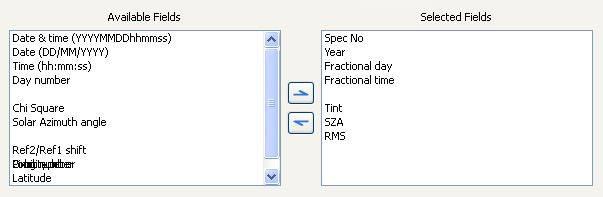
\includegraphics[width=\textwidth]{img/TroubleShooting_Output.jpg}
\end{minipage}
\end{figure}
\FloatBarrier

In the \textbf{Display} and the \textbf{Output pages} of \textbf{Projects properties}, the list of available fields that can be selected for display or output depend on the file format.  There is a problem with the refreshing of the list (missing fields or overwritten fields) after the selection of a new instrument or file format.  The list is correctly refreshed after quitting the \textbf{Projects properties} dialog box on \textbf{OK} and load it again.

All selected fields in the output page will be in the \textbf{output file} but some selected fields in the \textbf{Display page} could still have no effect on the display in the \textbf{Data page}.

\section{Analysis problems}\label{sec:analysis-problems}

\subsection{Calibration problems}\label{sec:calibration-problems}

Most problems usually come from the original wavelength calibration of the reference spectrum.  QDOAS corrects small shifts but the \gls{nlls} algorithm may not converge if the initial values are too far away from the solution (convergence to a local minimum of the chi-square).   Before using QDOAS, it is recommended to determine the preliminary wavelength calibration with a mercury lamp or to pre-convolve a solar spectrum at the resolution of your instrument, plot it with your spectrum and fit a polynomial through some pixels/nm couples set from the most representative Fraunhofer lines.  In the example below, even if the calcium lines match between the reference spectrum and the solar spectrum convolved at the resolution of the instrument, we can see that the wavelength calibration is completely wrong below 380 nm.  The differences are too large for QDOAS and it is better to correct that manually before running the calibration procedure.

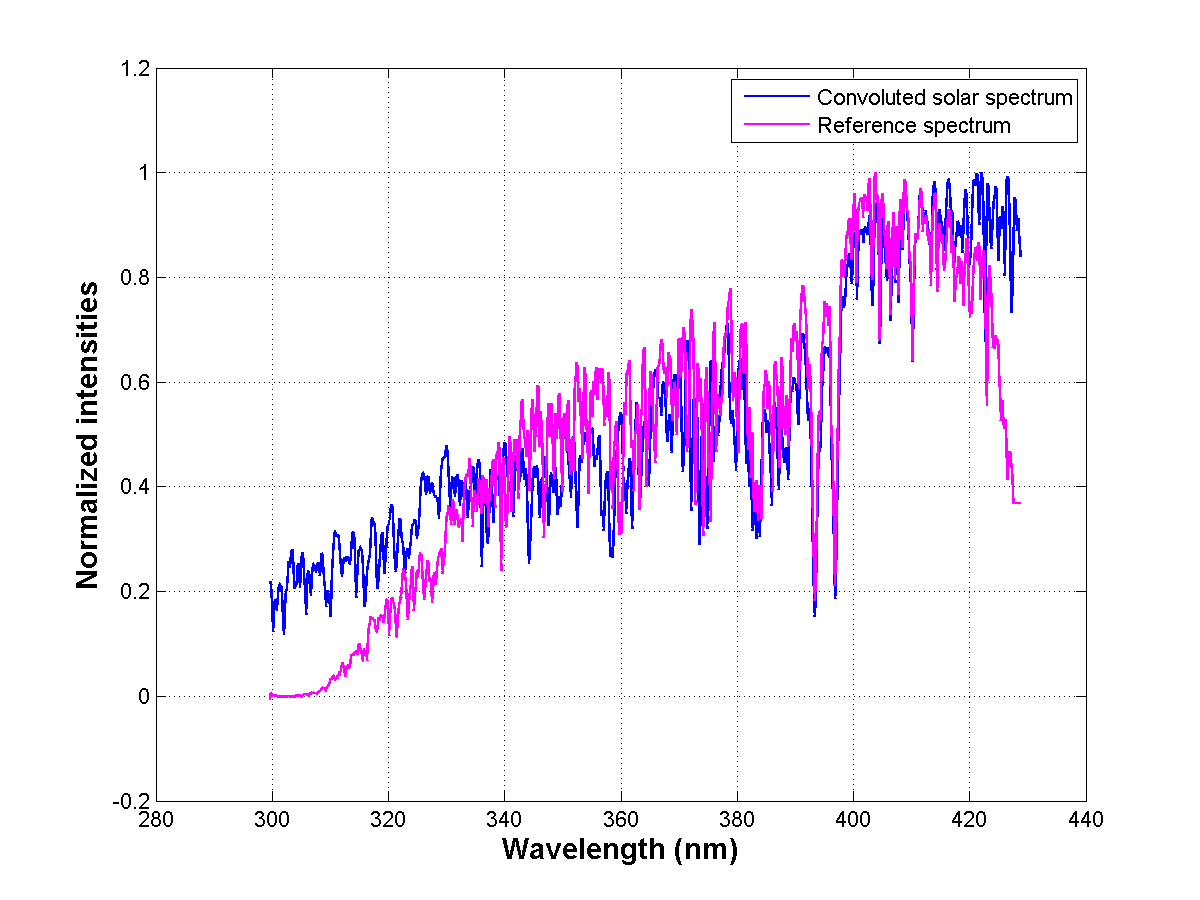
\includegraphics[width=\textwidth]{img/TroubleShooting_Calibration.jpg}

\subsection{Analysis error messages}

\textbf{Log error :}

\hspace{1cm}\parbox{11.5cm}{This message occurs mainly when the signal of the spectrum is too poor.  Usually, the message can be ignored if the cause can be identified : poor light conditions during twilight... If this error is systematic, the fit of a linear offset can be preferred to a non linear one (see page \pageref{eq:linear_offset}) or the fitting interval can be adjusted to another region where the signal is higher.}

\textbf{Sqrt argument error :} \\
\textbf{Curfit error :} \\
\textbf{Ill-conditioned matrix :}
\vskip 6pt
\hspace{1cm}\parbox{11.5cm}{These two messages are usually related to a problem with the configuration.

Check that all cross sections are defined in the fitting interval.  This can be done by right-clicking the \textbf{``View cross sections''} option from the analysis windows items.

Eventually, reduce the number of fitting parameters to the minimum (just the polynomial) and proceed step by step in order to identify the problem.

If the problem occurs during the calibration procedure, report to the section \textbf{``Calibration problems''} above.}

\textbf{Allocation error during the Kurucz procedure :}

\hspace{1cm}\parbox{11.5cm}{The degree of the polynomial fitting the continuous part of spectrum has not been defined in the \textbf{``Linear parameters page''} (see \textbf{Calibration page} of \textbf{Projects Properties}, page \pageref{sec:projects_calibration_page}).}

\textbf{spline interpolation requests increasing abscissae (...) :}

\hspace{1cm}\parbox{11.5cm}{The problem can come from a bad input file (preliminary wavelength calibration in the \textbf{``Instrumental page''} of \textbf{Projects properties}, cross section, reference spectrum) or the wavelength calibration procedure doesn't succeed to correct the preliminary wavelength calibration (report to the section \textbf{``Calibration problems''} above).}

\textbf{Number of degree of freedom $<=$ 0... :}

\hspace{1cm}\parbox{11.5cm}{Too many parameters are fitted w.r.t. the size of the fitting interval or the settings of the filter are not suitable.  Reduce the number of parameters to fit, increase the fitting interval or adjust the size of the filter.  Check also the calibration settings (Calibration page of Projects Properties).}

\textbf{Cross section file is empty or not large enough :}

\hspace{1cm}\parbox{11.5cm}{Check that all cross sections are defined in the fitting interval.  This can be done by right-clicking the \textbf{``View cross sections''} option from the analysis windows items.   Do not also forget the cross sections and the solar spectrum defined in the Calibration page of Projects Properties.}

%%% Local Variables: 
%%% mode: latex
%%% TeX-master: "QDOAS_manual"
%%% TeX-PDF-mode: t
%%% End: 

